\documentclass{standalone}

\usepackage{tikz}
\usepackage{pgfplots}

\begin{document}

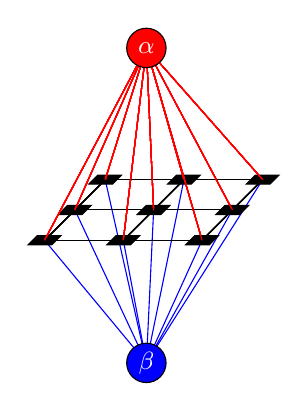
\begin{tikzpicture}

\def\dist{1}
\def\radi{0.25}
\def\squ{0.3}
\def\d{1.5}
\def\a{3.5}
\def\b{-3.5}





%blue edges
\foreach \i in{0, 1 ,2, ..., 2}{
    \foreach \j in{0,1, 2, ..., 2}{
        \draw [color=blue](\i+\squ/2,0 , \j+\squ/2) -- (1,-2,1);
    }
}



%pixel
\foreach \i in{0, 1 ,2, ..., 2}{
    \foreach \j in{0,1, 2, ..., 2}{
        \draw[fill] (\i,0,\j) -- (\i+\squ, 0,\j) -- (\i+\squ,0,\j+\squ) --(\i,0, \j+\squ) --cycle;


\draw (0+\squ/2, 0, \squ/2) -- (1+\squ/2, 0, \squ/2);
\draw (1+\squ/2, 0, \squ/2) -- (2+\squ/2, 0, \squ/2);
\draw (0+\squ/2, 0, 1+\squ/2) -- (1+\squ/2, 0, 1+\squ/2);
\draw (1+\squ/2, 0, 1+\squ/2) -- (2+\squ/2, 0, 1+\squ/2);
\draw (0+\squ/2, 0, 2+\squ/2) -- (1+\squ/2, 0, 2+\squ/2);
\draw (1+\squ/2, 0, 2+\squ/2) -- (2+\squ/2, 0, 2+\squ/2);

\draw (0+\squ/2, 0, \squ/2) -- (0+\squ/2, 0, 1+\squ/2);
\draw (1+\squ/2, 0, \squ/2) -- (1+\squ/2, 0, 1+\squ/2);
\draw (2+\squ/2, 0, \squ/2) -- (2+\squ/2, 0, 1+\squ/2);
\draw (0+\squ/2, 0,1+ \squ/2) -- (0+\squ/2, 0, 2+\squ/2);
\draw (1+\squ/2, 0,1+ \squ/2) -- (1+\squ/2, 0, 2+\squ/2);
\draw (2+\squ/2, 0,1+ \squ/2) -- (2+\squ/2, 0, 2+\squ/2);



%red edges
\foreach \i in{0, 1 ,2, ..., 2}{
    \foreach \j in{0,1, 2, ..., 2}{
        \draw[color=red] (\i+\squ/2,0 , \j+\squ/2) -- (1,2,1);
    }
}



    }
}

% \foreach \i in{0, 1 }{
%     \foreach \j in{0,1}{
%         \draw (\i+\squ,0, \j+\squ) --  (2*\i, 0, j);
%         % \draw[fill] (\i,0,\j) -- (\i+\squ, 0,\j) -- (\i+\squ,0,\j+\squ) --(\i,0, \j+\squ) --cycle;
%     }
% }


% \def\i{0}
% \def\j{0}
% \draw (\i,0,\j) -- (\i+\squ, 0,\j) -- (\i+\squ,0,\j+\squ) --(\i,0, \j+\squ) --cycle;
% \draw (\i+\squ/2,0 , \j+\squ/2) to[in=240, out=90](\i+0.4, 1, \j+0.4) to[out=60, in=60](1,2,1);
% \draw (\i+\squ/2,0 , \j+\squ/2) to[in=240, out=90](\i+0.4, -2, \j+0.4) to[out=60, in=60](1,-2,1);
% \draw (\i+\squ/2,0 , \j+\squ/2) -- (1,-2,1);

% \def\i{0}
% \def\j{1}
% \draw (\i,0,\j) -- (\i+\squ, 0,\j) -- (\i+\squ,0,\j+\squ) --(\i,0, \j+\squ) --cycle;
% % \draw (\i+\squ/2,0 , \j+\squ/2) --(1,2,1);
% % \draw (\i+\squ/2,0 , \j+\squ/2) -- (1,-2,1);

% \def\i{0}
% \def\j{2}
% \draw (\i,0,\j) -- (\i+\squ, 0,\j) -- (\i+\squ,0,\j+\squ) --(\i,0, \j+\squ) --cycle;
% % \draw (\i+\squ/2,0 , \j+\squ/2) --(1,2,1);
% % \draw (\i+\squ/2,0 , \j+\squ/2) -- (1,-2,1);

% \def\i{1}
% \def\j{0}
% \draw (\i,0,\j) -- (\i+\squ, 0,\j) -- (\i+\squ,0,\j+\squ) --(\i,0, \j+\squ) --cycle;
% % \draw (\i+\squ/2,0 , \j+\squ/2) --(1,2,1);
% % \draw (\i+\squ/2,0 , \j+\squ/2) -- (1,-2,1);

% \def\i{1}
% \def\j{1}
% \draw (\i,0,\j) -- (\i+\squ, 0,\j) -- (\i+\squ,0,\j+\squ) --(\i,0, \j+\squ) --cycle;
% % \draw (\i+\squ/2,0 , \j+\squ/2) --(1,2,1);
% % \draw (\i+\squ/2,0 , \j+\squ/2) -- (1,-2,1);

% \def\i{1}
% \def\j{2}
% \draw (\i,0,\j) -- (\i+\squ, 0,\j) -- (\i+\squ,0,\j+\squ) --(\i,0, \j+\squ) --cycle;
% % \draw (\i+\squ/2,0 , \j+\squ/2) --(1,2,1);
% % \draw (\i+\squ/2,0 , \j+\squ/2) -- (1,-2,1);



% %labels
\draw[fill=red] (1,2,1) circle (\radi) node{\textcolor{white}{\small$\alpha$}}; 
\draw[fill=blue] (1,-2,1) circle (\radi) node{\textcolor{white}{\small $\beta$}}; 




\end{tikzpicture}

\end{document}
